\documentclass[pdf]{beamer}

\mode<presentation>{}


%% preamble
\title[Конкурс молодых ученых]{Учет неразрешенных двойных звезд при оценивании массы РЗС}


\author[Бородина О. И.]{Бородина О. И.\textsuperscript{1} \and Селезнев А. Ф.\textsuperscript{1} \\  Карраро Дж.\textsuperscript{2} \and  Данилов В. М.\textsuperscript{1}}

\institute[]{\textsuperscript{1}Ural Federal University, Ekaterinburg, Russia \and \inst{2} Dipartimento di Fisica e Astronomia, Universit\'a di Padova Vicolo Osservatorio}


\date[\today] % (optional)
{Конкурс молодых ученых,\\ ИНАСАН, 2019}
\usetheme{CambridgeUS}
\usecolortheme{seahorse}
\useoutertheme{infolines}
\useinnertheme{rounded}
\usepackage{longtable}
\usepackage{xfrac}

\usepackage{tikz}
\usetikzlibrary{positioning}
\usetikzlibrary{shapes.geometric}
\usepackage{amsmath,amsfonts,amstext,amssymb}
\usepackage[english,russian]{babel}


\tikzstyle{rectangle1} = [rectangle, rounded corners, minimum width=4cm, minimum height=1cm, text centered, draw=black, fill=black!0, very thick]

\tikzstyle{rectangle2} = [rectangle, rounded corners, minimum width=2cm, minimum height=1cm, text centered, draw=black, fill=black!4, very thick]

\tikzstyle{rectangle3} = [rectangle, rounded corners, minimum width=4cm, minimum height=1cm, text centered, draw=black, fill=blue!10, very thick]

\begin{document}
  	%% title frame
	\begin{frame}
	    \titlepage
	\end{frame}
	
	%% 2
	\begin{frame}{Проблема}
	  \begin{itemize}
	  	\item При одинаковом потоке от одиночной и двойной $L_s = L_1 + L_2$
	  	\item Масса одиночной звезды меньше $M_s < M_1 + M_2$
	  	\item Следует корректировать массу скопления 
	\end{itemize}
	
	\vspace{0.3cm}
	\centering
	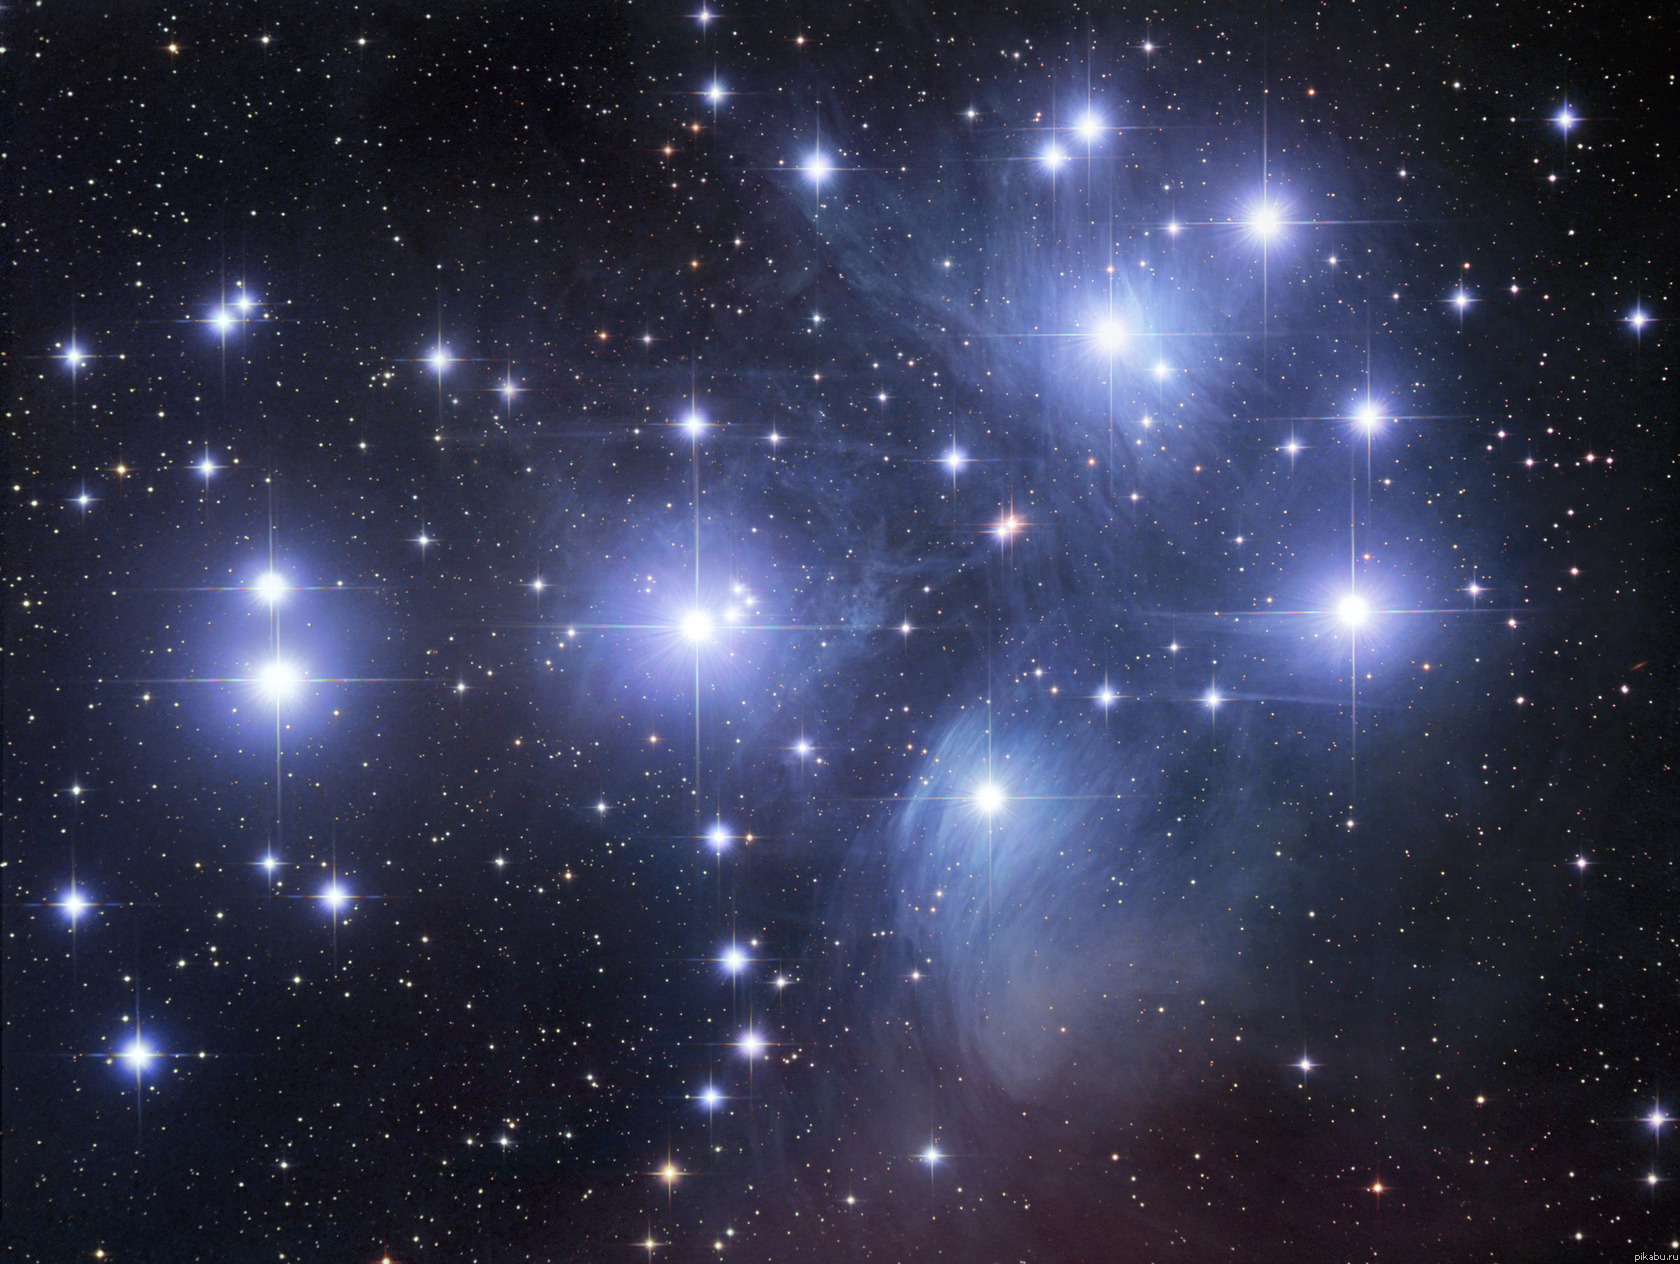
\includegraphics[width=6.5cm]{images/pleiades.jpg}
	\end{frame}
	
	%% 3
	\begin{frame}{Постановка задачи}
		Определить:
	    \begin{itemize}
	  	\item От чего зависит поправка к массе скопления
	  	\item Отличие поправочного коэффициента для разных скоплений
		\end{itemize}

	
	\end{frame}
	
	%% 4
	\begin{frame}{Параметры, определяющие поправку к массе}
		\begin{itemize}
			\item Зависимость доли двойных от звездной величины
			\item Вид распределения параметра $ q = \sfrac{\mathfrak{M_2}}{\mathfrak{M_1}} $
		\end{itemize}
		\pause

		\begin{columns}
			\begin{column}{0.47\textwidth}
			\begin{itemize}
				\item[--] Два гауссова распределения
				\item[--] Плоское распределение
				\item[--] Случай одинаковых компонент двойных
				\item[--] Случай одинаковых компонент кратных в  заданном численном соотношении$^1$
				
			\end{itemize}	
			\hspace{0.2cm}	
			{\footnotesize $^1$ Tokovinin (2014)}
			\end{column}
			
			\begin{column}{0.5\textwidth}
				
				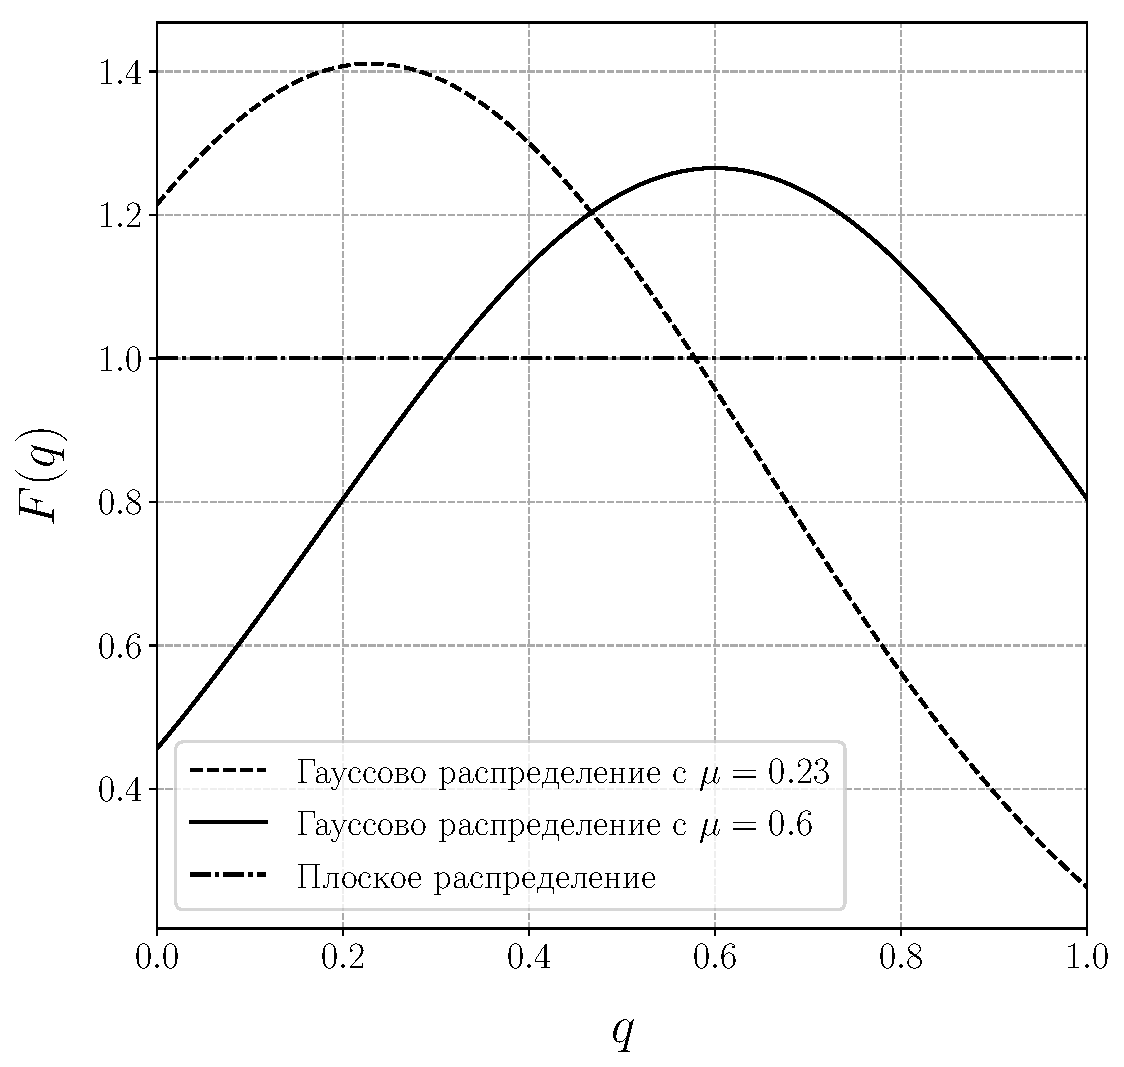
\includegraphics[width=5cm]{images/q_dists.pdf}
			\end{column}
		\end{columns}
		\vspace{-0.5cm}

	\end{frame}
	
	%% 5
	\begin{frame}{Выбор метода моделирования двойной}

		Методы моделирования двойной:
		\vspace{1cm}
		
		\centering
		\begin{tikzpicture}
			\node[rectangle1, align=center](maintopic){Функция масс};
			\node[rectangle1, right=of maintopic](1){Распределение по $q$};	
			\hspace{-1.5cm}
			\node[rectangle2, below right=of maintopic](2){$\mathfrak{M_1}, \mathfrak{M_2}$};
			\draw[->, line width=1.5] (1.4,-0.5) to (3.05,-1.55);
			\draw[->, line width=1.5] (6.5,-0.5) -- (5.02,-1.55);
		\end{tikzpicture}
		
		\raggedright
		\vspace{0.5cm}
		
		\begin{minipage}[height=2cm]{15cm} 
			   {\footnotesize Kouwenhoven et al. (2009)}
		\end{minipage}
	\end{frame}
	
	
	%% 6
	\begin{frame}{Выбор метода моделирования двойной}

		Методы моделирования двойной:
		\vspace{1cm}
		
		\centering
		\begin{tikzpicture}
			\node[rectangle3, align=center](maintopic){Функция светимости};
			\node[rectangle1, right=of maintopic](1){Распределение по $q$};	
			\hspace{-1.5cm}
			\node[rectangle2, below right=of maintopic](2){$\mathfrak{M_1}, \mathfrak{M_2}$};
			\draw[->, line width=1.5] (1.4,-0.5) to (3.05,-1.55);
			\draw[->, line width=1.5] (6.5,-0.5) -- (5.02,-1.55);
		\end{tikzpicture}
		
		\raggedright
		\vspace{0.5cm}
		\begin{minipage}[height=2cm]{15cm} 
		
			 \onslide<2->{Наша задача требует {\bfseries нового} метода!}
		\end{minipage}
	\end{frame}
	
	%% 7
	\begin{frame}{Входные данные}
		\begin{columns}
			\begin{column}{0.6\textwidth}
   				\begin{itemize}
					\item Функция светимости ЗС
					\item<2-> Зависимость масса-светимость $^1$
				\begin{equation*} \hspace{-1.5cm}
				\log L=a \cdot (\log\mathfrak{M})^2+b \cdot \log\mathfrak{M}+c
				\end{equation*}
					\item<3-> Таблица изохроны $^2$
				\end{itemize}
			\end{column}
			
			\begin{column}{0.8\textwidth}
				\hspace{-0.5cm}
    			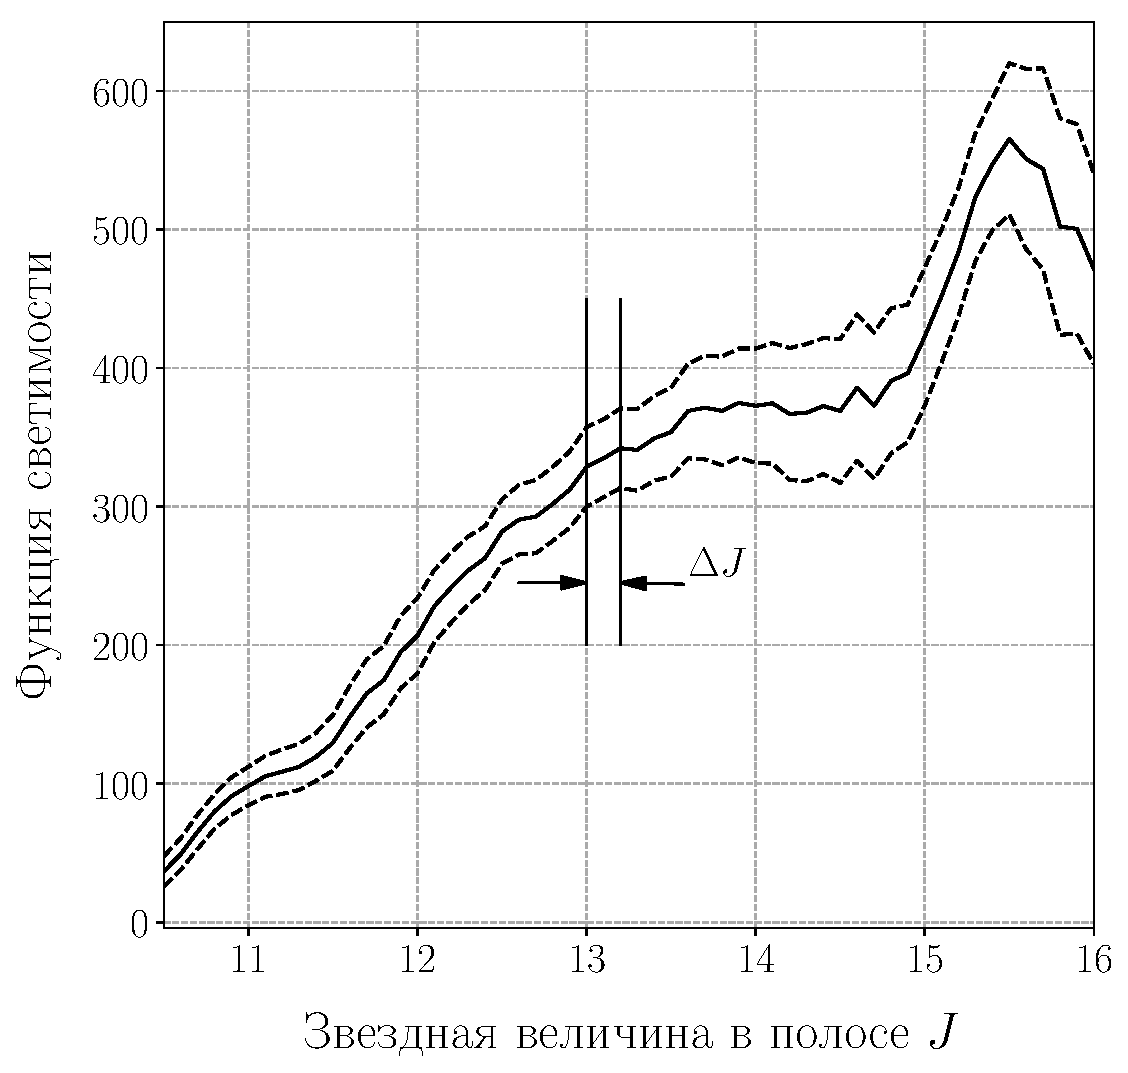
\includegraphics[width=5cm]{images/LF}
			\end{column}
		\end{columns}
		
		\vspace{1cm}
		\onslide<2-> {\footnotesize $^1$ Eker et al. (2015)}
		
		\onslide<3-> {\footnotesize $^2$ Bressan et al. (2012)}
	\end{frame}
	
	%% 8
	\begin{frame}{Список скоплений}
	\centering
		\begin{tabular}{|c|c|c|c|c|}
			\hline
				\bf{Скопление} & \bf{Интервал по J}& $\bf{(m-M)_0}$ & \bf{E(B-V)} & $\bf{log(t)}$\\
			\hline
			IC2714 & [10.5; 16.0] & 10.48 & 0.34 & 8.6\\
			NGC1912 & [9.8;  16.0] & 10.29 & 0.25 & 8.3\\
			NGC2099 & [10.5;  16.0] & 10.74 & 0.30 & 8.7\\
			NGC6834 & [11.0;  15.9] & 11.59 & 0.71 & 7.9\\
			NGC7142 & [11.2;  16.0] & 10.2 & 0.25 & 9.2\\
			\hline
		\end{tabular}
	\end{frame}
	
	%% 9
	\begin{frame}{Описание метода}
		\begin{itemize}
			\item Задаем долю двойных $\alpha$
			\item Считаем $N_{binaries}$ для каждого интервала $\Delta J$
			\item Для всех звезд определяем светимость $L$ 
			\item Для каждой двойной определяем $q$ (метод Неймана)
		
			\pause
			\item Определяем $\mathfrak{M_1}$ и $\mathfrak{M_2}$ из СУ:
		\end{itemize}
		
		\[		
		\left\{ 
			\begin{array}{l}
				L=L_1+L_2 \\
				\log(L_1)=a*(\log\mathfrak{M}_1)^2+b*\log\mathfrak{M}_1+c\\
				\log(L_2)=a*(\log\mathfrak{M}_2)^2+b*\log\mathfrak{M}_2+c \\
				q = \sfrac{\mathfrak{M_2}}{\mathfrak{M_1}}
			\end{array}
		\right.
		\]
		\begin{itemize}
			\item Находим массу всех двойных звезд ЗС
		\end{itemize}
	\end{frame}

	
	%% 10
	\begin{frame}{Результаты}
		\begin{columns}
			\begin{column}{0.45\textwidth}
				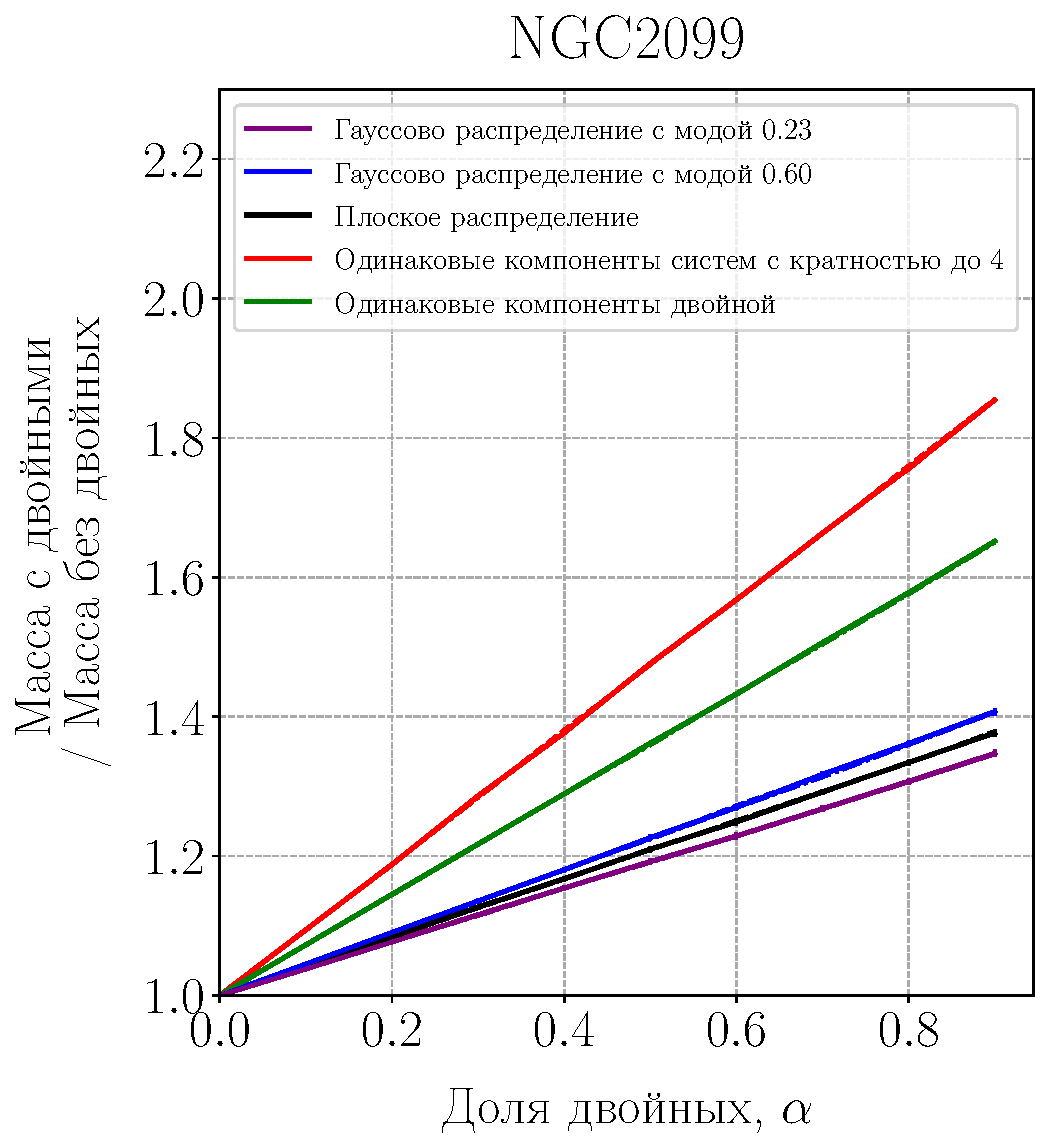
\includegraphics[width=5.5cm]{images/alphas_NGC2099}
			\end{column}
			
			\begin{column}{0.5\textwidth} 
    			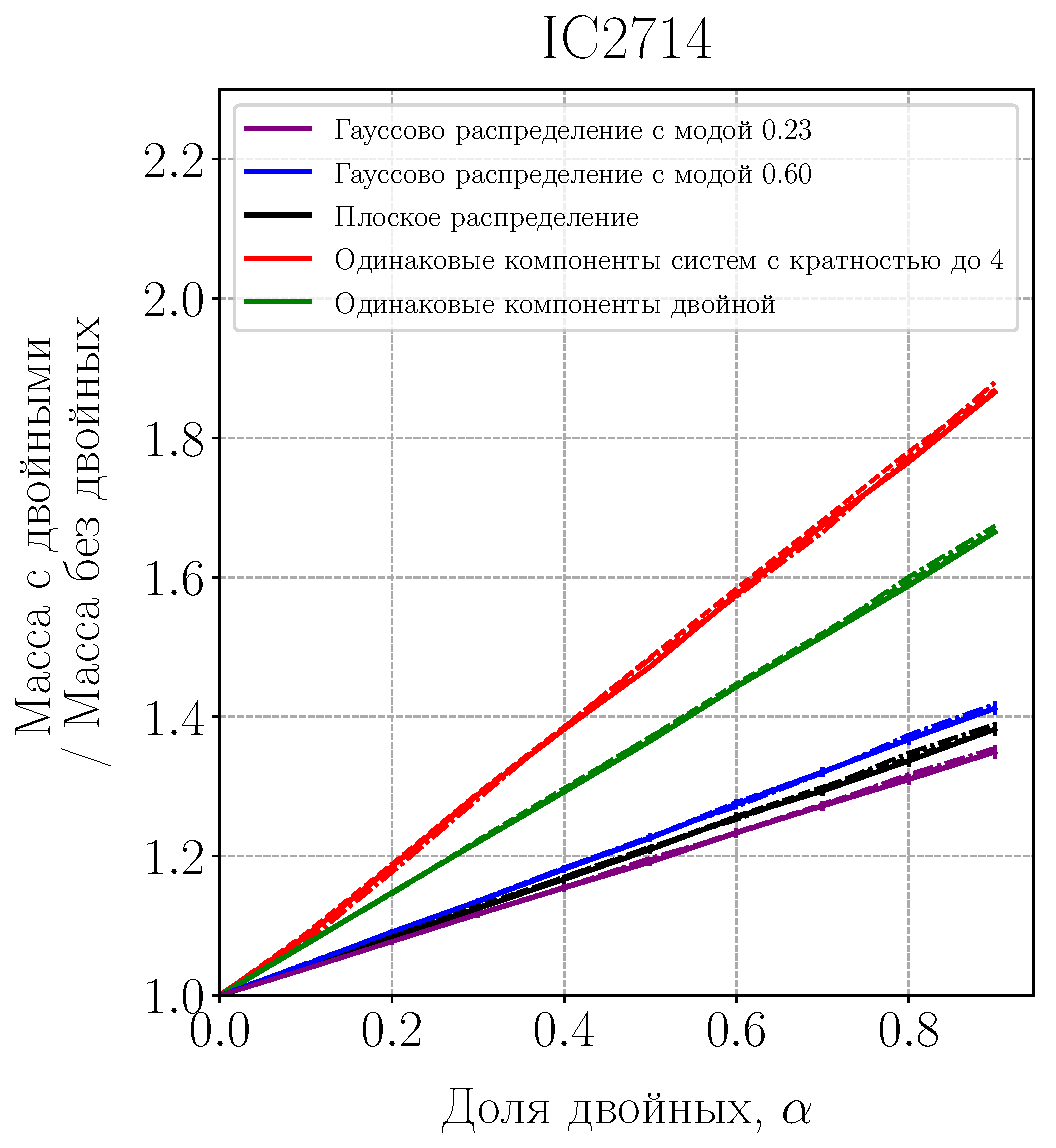
\includegraphics[width=5.5cm]{images/alphas_IC2714}
			\end{column}
		\end{columns}
	\end{frame}
	
	%% 11
	\begin{frame}{Результаты}
	\centering
		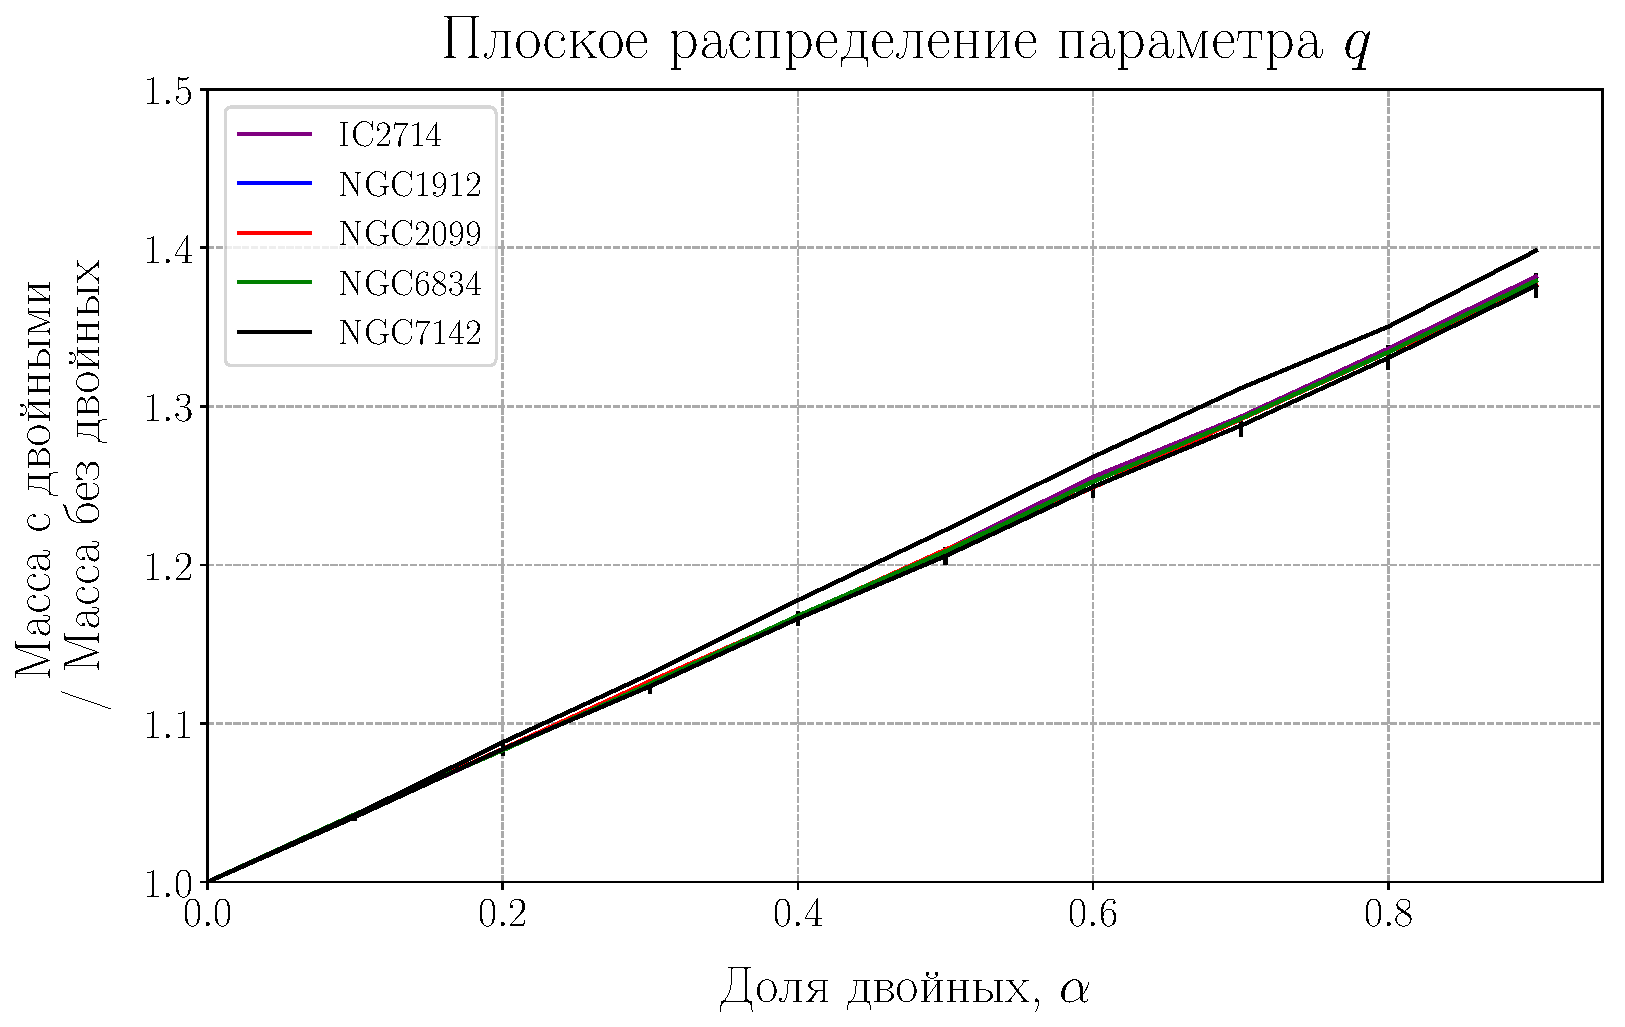
\includegraphics[width=10cm]{images/alphas_flat}
	\end{frame}
	
	%% 12
	\begin{frame}{Выводы}
		\begin{itemize}
			\item Полученные зависимости -- {\bf линейные}
			\item Чем ближе максимум распределения по $q$ к 1, тем больше поправочный коэффициент.
			\item Вид функции светимости значительно {\bf не влияет} на значение поправочного коэффициента.
			\item Для <<реалистичных>> распределений поправка к массе отличается {\bf незначительно}.
		\end{itemize}
		
	\vspace{2cm}

	{\footnotesize Borodina et.al  <<Unresolved Binaries and Galactic Clusters’ Mass Estimates>> (2019)}
	\end{frame}



	
\end{document}
